\documentclass[tikz]{standalone}
\usepackage{pgfplots}
\pgfplotsset{compat=1.15}
\usepackage{mathrsfs}
\usetikzlibrary{arrows,calc}
\usepackage{tkz-euclide}
\pagestyle{empty}

\definecolor{AngleClr}{rgb}{0,0.39215686274509803,0}
\definecolor{ShapeClr}{rgb}{0.6,0.2,0}
\definecolor{BlueSqr}{RGB}{5,81,163}
\definecolor{RedSqr}{RGB}{0, 156, 0}

\newcommand{\add}[2]{\dimexpr#1+#2\relax}

\begin{document}

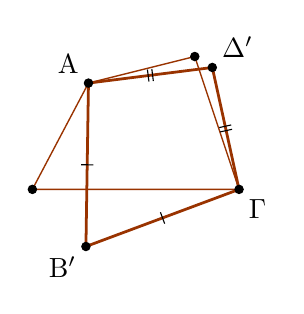
\begin{tikzpicture}[scale=.75]
\tkzSetUpLine[line width=1pt,color=black]
\tkzSetUpPoint[fill=black]

\tkzDefPoints{0/0/B,3.5/0/C,0.95/1.8/A,2.75/2.25/D}

\tkzCalcLength(A,B)\tkzGetLength{dAB}
\tkzCalcLength(C,B)\tkzGetLength{dCB}

\tkzCalcLength(A,D)\tkzGetLength{dAD}
\tkzCalcLength(C,D)\tkzGetLength{dCD}

\pgfmathsetmacro{\dOne}{(\dAB+\dCB)/2}
\pgfmathsetmacro{\dTwo}{(\dAD+\dCD)/2}

% \tkzInterCC[R](A,(\dAB + \dCB)/2)(C,(\dAB + \dCB)/2) \tkzGetPoints{X}{Y}
\tkzInterCC[R](A,\dOne)(C,\dOne) \tkzGetPoints{X}{B'}
\tkzInterCC[R](A,\dTwo)(C,\dTwo) \tkzGetPoints{D'}{Y}

\tkzFillPolygon[fill=white](A,B,C,D)
\tkzFillPolygon[fill=white](A,B',C,D')

\tkzDrawPolygon[color=ShapeClr,line width=0.5pt](A,B,C,D)
\tkzDrawPolygon[color=ShapeClr](A,B',C,D')
\tkzDrawPoints[size=3](A,B,C,D,B',D')
\tkzLabelPoint[above left](A){$\rm A$}
\tkzLabelPoint[below left](B'){$\rm B'$}
\tkzLabelPoint[below right](C){$\rm \Gamma$}
\tkzLabelPoint[above right](D'){$\rm \Delta'$}

\tkzMarkSegments[mark=||,size=2.2](A,D' C,D')
\tkzMarkSegments[mark=|,size=2.2](A,B' C,B')

\end{tikzpicture}

\end{document}
